\chapter{Implementacja}

Głównym założeniem projektu było stworzenie go w taki sposób, aby kod jak najtrafniej odzwierciedlał rzeczywistość. W tym celu stworzono klasy obiektów reprezentujące rzeczywiste byty w świecie realnym.
\begin{figure}[H]
\centering
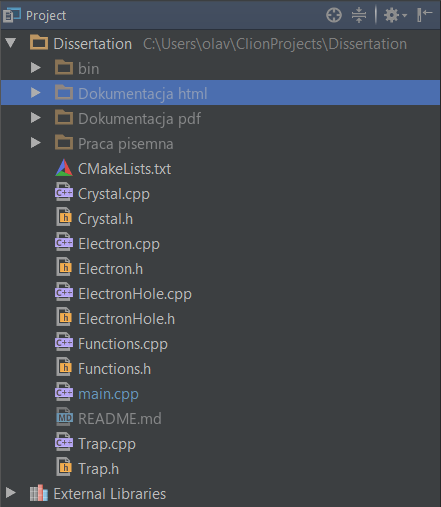
\includegraphics[width=15cm]{strukturaprojektu}
\caption{Struktura projektu.}
\label{fig:Struktura projektu}
\end{figure}
\section{Klasy}
Każda z klas posiada własne metody w zależności od swojego przeznaczenia.

Klasa \textit{Electron} odzwierciedla cząstkę elementarną - elektron. Zmiana ilości tych cząstek w stanie wzbudzonym tj. znajdujących się w pułapce jest głównym celem wykonania tej symulacji.

\textit{ElectronHole} jest reprezentacją dziury elektronowej, z którą to elektron po wykorzystaniu zjawiska tunelowego zrekombinuje.

Klasa \textit{Trap} odpowiada defektom w sieci krystalicznej czyli pułapkom, które mogą przechwycić elektron lub dziurę elektronową.
Na potrzeby wykonania tej symulacji założono, że na samym jej początku wszystkie obiekty reprezentujące elektrony oraz dziury elektronowe znajdują się już w pułapkach. Dodatkowo, w symulacji ustalono, że dany elektron jeśli spełni warunek wystąpienia zjawiska tunelowego - po jego zajściu i rekombinacji z dziurą - nie może przetunelować ponownie. Zostało to podyktowane zmniejszeniem oczekiwanego czasu działania programu.

Klasa \textit{Crystal} reprezentuje rzeczywisty kryształ, który będzie poddany symulacji zaniku sygnału luminescencyjnego. Zawiera on w sobie inne obiekty takie jak:

\begin{itemize}
\item Elektrony
\item Dziury elektronowe
\item Obiekty odpowiadające defektom sieci krystalicznej - tzw. pułapki
\end{itemize}

\section{Opis działania programu}



W celu otrzymania danych niezbędnych do wygenerowania wykresu zależności między ilością elektronów w pułapkach a upływem czasu uruchomiono stworzony program. Obiekt \textit{Crystal} w swoim konstruktorze generuje podaną ilość dziur elektronowych, pułapek oraz elektronów, a następnie przechowuje je w oddzielnych kontenerach. Dla każdej z tych cząstek wywoływany jest konstruktor (ustawiający współrzędne położenia) z argumentami, które są losowane z podanego wcześniej przedziału (wartości są podane w Angstremach tj. 1 Å = $10^{-10}$m. Jednostka ta nie jest jednostką układu SI, lecz jest stosowana w fizyce przy opisywaniu obiektów i zjawisk zachodzących w skali atomowej). Jak podkreślono wcześniej, symulacja zakłada, że na jej starcie każdy elektron znajduje się w pułapce. Powoduje to, że para elektron - pułapka ma identyczne współrzędne położenia, a także obiekt klasy \textit{Trap} przyjmuje wskaźnik na uwięziony w nim elektron.

Następnie za pomocą metody \textit{startSimulation(int time)} obiektu klasy \textit{Crystal} rozpoczynana jest symulacja. Symulowany upływ czasu  zależy od wartości argumentu \textit{time}, który jest wyrażony w dniach tj. wywołanie \emph{startSimulation(365)} oznacza rozpoczęcie działania symulacji symulującej efekt zaniku sygnału luminescencyjnego w czasie 1 roku.

Podczas wykonywania symulacji każda pułapka elektronowa jest sprawdzana czy przechowuje w sobie uwięziony elektron. Jeśli warunek jest spełniony, to dla elektronu oraz dziur elektronowych znajdujących się w pułapkach ,za pomocą wzoru (1.1) sprawdzane jest prawdopodobieństwo zajścia efektu tunelowego. Jeśli ma ono miejsce elektron opuszcza swoją pułapkę (wskaźnik obiektu klasy \textit{Trap} na elektron ustawiany jest na wartość \textit{NULL}), a następnie zmienia swoje dotychczasowe położenie na współrzędne do których przetunelował (współrzędne centrum rekombinacyjnego/dziury). Powtarzane jest to tak długo, aż program za symuluje podany mu wcześniej czas trwania symulacji.  Jak wynika z założeń projektu wspomnianych wcześniej - jeśli elektron przetunelował do centrum rekombinacji przynajmniej raz, nie będzie on brał więcej udziału w obliczaniu prawdopodobieństwa zajścia efektu tunelowego. 

Po skończeniu symulacji, program zapisuje do pliku otrzymane wyniki w formacie \textit{czas;ilość elektronów w stanie wzbudzenia}, gdzie czas wyrażony jest w $ \log(\frac{t}{2 dni}) $, a ilość elektronów jest kwantowana do 1. Za pomocą skryptu \textit{wykres.plt}
w folderze \textit{bin/Debug} generowany jest odpowiedni wykres ilustrujący otrzymane dane. 

Przykładowo wygenerowany wykres (analiza otrzymanych wykresów znajduje się w dalszej części pracy):

\begin{figure}[H]
\centering
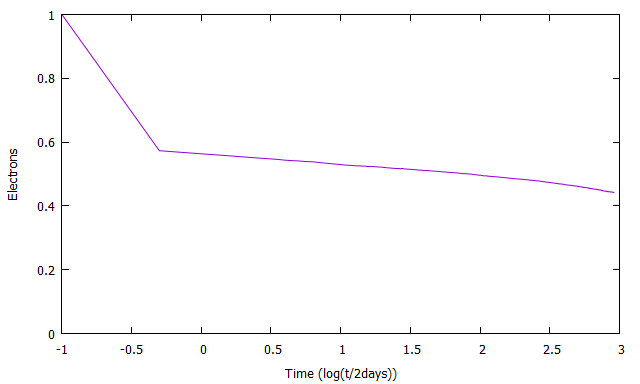
\includegraphics[width=15cm]{example}
\caption{Przykładowa wizualizacja otrzymanych danych}
\label{fig:example}
\end{figure}

